\documentclass{article}

\usepackage{ctex}
\usepackage{tikz}
\usetikzlibrary{cd}

\usepackage{amsthm}
\usepackage{amsmath}
\usepackage{amssymb}

%\usepackage{unicode-math}


\usepackage[textwidth=18cm]{geometry} % 设置页宽=18

\usepackage{blindtext}
\usepackage{bm}
\parindent=0pt
\setlength{\parindent}{2em} 
\usepackage{indentfirst}

\usepackage{listings}
%\usepackage{minted}% hightlighting

\usepackage{proof} % infer

\usepackage{xcolor}
\usepackage{titlesec}
\titleformat{\section}[block]{\color{blue}\Large\bfseries\filcenter}{}{1em}{}
\titleformat{\subsection}[hang]{\color{red}\Large\bfseries}{}{0em}{}
%\setcounter{secnumdepth}{1} %section 序号

\newtheorem{theorem}{Theorem}[section]
\newtheorem{lemma}[theorem]{Lemma}
\newtheorem{corollary}[theorem]{Corollary}
\newtheorem{proposition}[theorem]{Proposition}
\newtheorem{example}[theorem]{Example}
\newtheorem{definition}[theorem]{Definition}
\newtheorem{remark}[theorem]{Remark}
\newtheorem{exercise}{Exercise}[section]
\newtheorem{annotation}[theorem]{Annotation}

\newcommand*{\xfunc}[4]{{#2}\colon{#3}{#1}{#4}}
\newcommand*{\func}[3]{\xfunc{\to}{#1}{#2}{#3}}

\newcommand\Set[2]{\{\,#1\mid#2\,\}} %集合
\newcommand\SET[2]{\Set{#1}{\text{#2}}} %

\begin{document}
\title{Abstract Interpretation}
\author{枫聆}
\maketitle
\tableofcontents

\section{Motivation}

实际分析domain太复杂,也许这个实际分析domain满足一些不错的性质比如ACC等等,但是还是掩盖不了它过于复杂. 所以我们尝试使用某个抽象的domain来代替分析,这个抽象的domain要比实际分析的domain更小,我们分析起来更加得心应手,但是问题是如何构造这个抽象的domain? 它分析出来的结果是否可以作为真的truth? 它的结果能在多大程度上说明一些问题? 后期我们是否可以考虑优化抽象的domain来让结果更好一点?

\newpage
\section{Galois connections}

关于galois connection我们通常可以看到两个定义,下面我来说明两个定义是等价,也就是说可以从任意一个推出另外一个.

\begin{definition}
\rm {\color{red} nlab上的定义更贴近adjunction的味道} Given posets $A$ and $B$, a Galois connection between $A$ and $B$ is a pair of order-preversing functions $\func{f}{A}{B}$ and $\func{g}{B}{A}$ such that $a \leq g(f(a))$ and $b \geq f(g(b))$ for all $a \in A$, $b \in B$. 

{\color{blue} 注意这里的order-preversing,最原始的定义用的是order-reversing,导致我在这里弄出了一些矛盾}.
\end{definition}

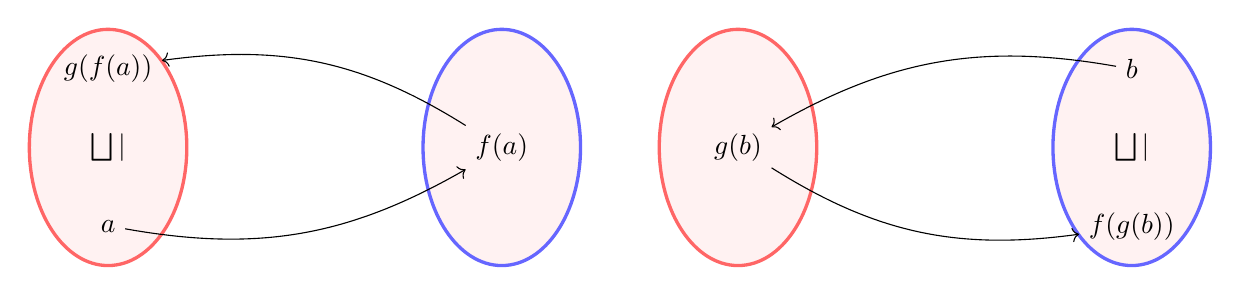
\begin{tikzpicture}
\filldraw[color=red!60, fill=red!5, very thick](-1,0) ellipse (1 and 1.5);
\filldraw[color=blue!60, fill=red!5, very thick](4,0) ellipse (1 and 1.5);
\node (a) at (-1,-1) {$a$};
\node (fa) at (4,0) {$f(a)$};
\node (gfa) at (-1, 1) {$g(f(a))$};
\node (l) at (-1,0) {$\bigsqcup|$};
\draw [->] (a) edge[bend right=20] (fa) (fa) edge[bend right=20] (gfa);

\filldraw[color=red!60, fill=red!5, very thick](7,0) ellipse (1 and 1.5);
\filldraw[color=blue!60, fill=red!5, very thick](12,0) ellipse (1 and 1.5);
\node (b) at (12, 1) {$b$};
\node (gb) at (7,0) {$g(b)$};
\node (fgb) at (12,-1) {$f(g(b))$};
\node (l) at (12,0) {$\bigsqcup|$};
\draw [->] (b) edge[bend right=20] (gb) (gb) edge[bend right=20] (fgb);
\end{tikzpicture}

\begin{proposition}
\rm Given posets $A$ and $B$, a pair of order-preversing functions $\func{f}{A}{B}$ and $\func{g}{B}{A}$ is a Galois connection between $A$ and $B$ if and only if, for all $a \in A$, $b \in B$, we have 
$$
f(a) \leq b~\text{if and only if}~a \leq g(b).
$$
\end{proposition}

\begin{center}
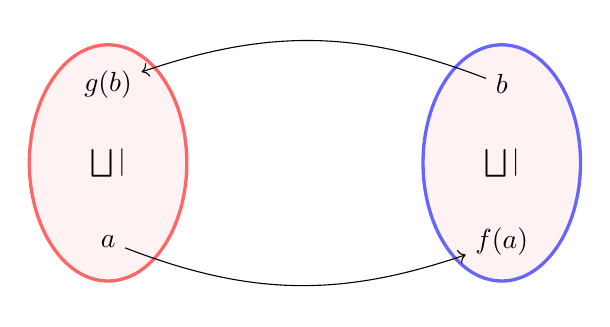
\begin{tikzpicture}
\filldraw[color=red!60, fill=red!5, very thick](-1,0) ellipse (1 and 1.5);
\filldraw[color=blue!60, fill=red!5, very thick](4,0) ellipse (1 and 1.5);
\node (a) at (-1,-1) {$a$};
\node (fa) at (4,-1) {$f(a)$};
\node (b) at (4, 1) {$b$};
\node (gb) at (-1,1) {$g(b)$};
\node (l1) at (-1,0) {$\bigsqcup|$};
\node (l2) at (4,0) {$\bigsqcup|$};
\draw [->] (a) edge[bend right=20] (fa) (b) edge[bend right=20] (gb);
\end{tikzpicture}
\end{center}

\begin{proof}
($\Rightarrow$). 前提$(f,g)$是一个galois connection,给定$a \in A$, $b \in B$. 若$f(a) \leq b$, 两边同时apply $g$, 有$g(f(a)) \leq g(b)$,同时有$a \leq g(f(a))$. 那么$a \leq g(b)$. 若$a \leq g(b)$,同理可以得到$f(a) \leq b$.

($\Leftarrow$). 前提$(f,g)$满足$f(a) \leq b~\text{if and only if}~a \leq g(b)$. 我们直接取$b = f(a)$, 那么$f(a) \leq f(b)$当且仅当$a \leq g(f(a))$. 同理直接取$a = g(b)$,那么$g(b) \leq g(b)$当且仅当$f(g(a)) \leq b $.   
\end{proof}

{\color{blue} 关于adjunction的东西$fg \rightarrow id$和$gf \rightarrow id$,这个箭头是一个natural transform, 至于更细的东西要去看看category theory了! PAAA上说$f$和$g$互为“weak inverse”,看起来也是比较形象啊!所以有下面的一个命题}.


\begin{proposition}
\rm {\color{red} weak inverse} For galois connection $(f,g)$, we have the equations
$$
\begin{aligned}
f \circ g \circ f  = f \\
g \circ f \circ g = g.
\end{aligned}
$$
\end{proposition}

\begin{proof}
(1).
$$
\begin{array}{ccc}
 a \leq g(f(a)) \Rightarrow& f(a) \leq f[g(f(a))] & {\color{red} f \circ( g \circ f)} \\
 f(a) \leq f(a) \Rightarrow& f\circ g(f(a))) \leq f(a) & {\color{red}(f \circ g) \circ f}, \\
\end{array}
$$
所以$f \circ g \circ f  = f$. 同理可证第二个式子.
\end{proof}

\begin{proposition}
\rm {\color{red} Galois connection引发的semilattice homomorphism} For a Galois connection $(f,g)$ of join semlattice $A$ and $B$, $f$ preserves finite join:
\begin{enumerate}
	\item $f(\perp) = \perp$;
	\item $f(x \vee y) = f(x) \vee f(y)$.
\end{enumerate}

{\color{blue} 啧啧,没想到啊galois connection竟然弄了一个semilattice homomorphism出来,突然想找一下characterization of semilattice homomorphism}. 
\end{proposition}

\begin{proof}
(1) 由于$B$上的$\perp$的性质,有$f(\perp) \geq \perp$. 反过来由于$A$上的$\perp$性质,有$g(\perp) \geq \perp$,再用一下galois connection的性质,有$f(\perp) \leq \perp$. 综上两边夹,所以$f(\perp) = \perp$.

(2) 由于$f$是monotone,有$f(x) \leq f(x \vee y)$和$f(x) \leq f(x \vee y)$,所以$f(x) \vee f(y) \leq f(x \vee y)$. 最关键的是证明$f(x \vee y) \leq f(x) \vee f(y)$. 由于galois connection,有$x \leq g(f(x))$,再由$g$是monotone,有$x \leq g(f(x) \vee f(y))$. 同理也有$y \leq g(f(x) \vee f(y))$,那么
$$
x \vee y \leq g(f(x) \vee f(y))
$$
再用一下galois connection,就有$f(x \vee y) \leq f(x) \vee f(y)$. 综上两边夹,所以$f(x \vee y) = f(x) \vee f(y)$.
\end{proof}

\newpage
\subsection{Inducing along the Concretisation Function}

\begin{definition}
\rm We shall say that the sequence $(x_1 \nabla \cdots \nabla x_n)_n$ {\color{red} eventaully stabilises} whenever there is a number $N$ such that $x_1 \nabla \cdots \nabla x_n = x_1 \nabla \cdots \nabla x_n \nabla x_{n+1}$ for all $n > N$.

{\color{blue} 这个$\nabla$表示widening,这个序列第$n$个元素是$n$个元素做apply widening之后的结果,最终会趋于稳定}.
\end{definition}

\begin{definition}
\rm An operator $\func{\nabla}{D \times D}{D}$ is a {\color{red} strong widening }whenever
\begin{itemize}
	\item $x_1 \nabla x_2 \geq x_1 \vee x_2$ holds for all $x_1,x_2 \in D$ and
	\item the sequence $(x_1 \nabla \cdots \nabla x_n)_n$ eventually stabilises for all choices of sequence $x_1, x_2 ,\cdots$.
\end{itemize}
\end{definition}

\begin{proposition}
\rm If $\nabla$ is a strong widening then
$$
x_1 \nabla \cdots \nabla x_n \leq x_1 \nabla \cdots \nabla x_n \nabla x_{n+1}
$$
for all $n > 0$.
\end{proposition}

\begin{proof}
当$n=1$时
$$
x_1 \leq x_1 \nabla x_2.
$$
这是显然地,假设对任意的$n = k$有$x_1 \nabla \cdots \nabla x_k \leq x_1 \nabla \cdots \nabla x_k \nabla x_{k+1}$成立,那么当$n = k+1$时
$$
\begin{aligned}
(x_1 \nabla \cdots \nabla x_k \nabla x_{k+1}) \nabla x_{k+2} &\geq (x_1 \nabla \cdots \nabla x_k \nabla x_{k+1}) \vee x_{k+2} \\
& \geq x_1 \nabla \cdots \nabla x_k \nabla x_{k+1}.
\end{aligned}
$$
所以原式在任意$n >0$时成立.
\end{proof}

\begin{proposition}
\rm If $D$ satisfies the ACC then the join operation $\vee$ is a strong widening.
\end{proposition}

\begin{proof}
这太显然了, 简直trivial,ACC在这里保证了任意非空集合都有最大元素,那么它们的join肯定不会超过它,也就是eventually stabilises.
\end{proof}



\end{document}
